\section{Model Class Implementations}
For various reasons described below, existing implementations of some models were not adequate for this research.
These reasons included speed, generality, and consistency.

\subsection{Model Execution: The Need for Speed}
Because optimization may involve an extremely large number of independent simulations of the same class of model, each varying only in model parameter values, it is critical that both the overhead for model instantiation and the duration of simulation itself, be as low as possible.
Existing modeling tools contain overhead associated with model initialization, shuttling results in memory, which are a trivial cost for single simulations, but begin to add up in optimization runs of thousands of simulations.  
Even the simulation of reduced models themselves are often slower than necessary using existing tools, due to some of these tools being written to accommodate more complex, biophysical models.
The speed of model simulation is often determined by the exact parameterization of the model in question.
During optimization, many parameter sets are explored. Those which produce many spikes in a given simulation run more slowly, because $\frac{dV_{M}}{dt}$ changes rapidly throughout the simulation and so simulation step size must sometimes be adaptively reduced to avoid numerical instability.

\subsection{Model Design: Lack of Generality}
Significant time was spent in the early years of this project shoe-horning pre-existing tools into the desired optimization framework, with limited success.
These tools included, among others, model designers and neural simulators such as PyNN, Brian2, NEURON, and jNeuroML.
However, several unexpected road blocks were encountered on the way.

\subsubsection{NEURON}
The \emph{NEURON} implementation of the Izhikevich model is fractured.
There are different implementations for different parameter regimes.
For a single simulation, this is not much of a problem.
However, it means that switching between such regimes during optimization (as would occur when a parameter value crossed a regime boundary), is a non-trivial exercise.
Even if successful, any source code successfully implementing this would be complicated, unreadable, and lack generality.
Specifically, NEURON requires NMODL files to be compiled for each different regime, and it may be difficult to know in advance which regimes the optimizer is likely to sample from.
Thus, the claimed performance of the C-based NEURON library is not actualized in an optimization context.
Because NEURON is well-understood within OSB and NeuroML community, I still used it only to produce reference simulations to verify that the output of my model implementations were in fact accurate.

\subsubsection{PyNN}
PyNN provides the convenience of working in Python, and with a convenient procedural interface for model design and execution.
However, its implementations of most reduced models (e.g. Izhikevich) are simply ``wrapped" versions of NEURON models; consequently PyNN has the same disadvantages as NEURON.
PyNN is also designed with network simulations in mind, which means its designers have chosen performance trade-offs that favor network simulations over single neuron simulations.
For example, a data-type called the ``lazy-array" is the most elemental container for neuron models in PyNN, but it is meant to store populations of neurons as opposed to single neurons;
as such the lazy-array can make accessing single model results complicated and confusing.

% in slow single neuron simulations.

Additionally the NEURON implementations that underlie the PyNN models of Adaptive Exponential and Izhikevich classes still suffer from some fidelity issues under certain regimes and parameter sets, the references are as follows: \url{https://github.com/NeuralEnsemble/PyNN/issues/370}, \url{https://github.com/NeuralEnsemble/PyNN/issues/266}, which optimization depends on.
% The above links should be turned into citations.

\subsubsection{Brian2}
Brian2 \citep{stimberg2019brian} is, in principle, an excellent simulator for working with reduced neuron models, as it allows for differential equations to be expressed in an intuitive form, while also keeping track of dimensions and units.
However, it may not quite be mature enough for complex applications, as it produced errors in optimization contexts that did not occur during routine simulation of single-parameter sets.

Even when these errors did not occur, (e.g. using the brian2/neuraldynamics AdExp model), certain optimization steps (such as identifying the rheobase current for a given set of model parameters) took 2-3 times more computation time.
This slowness was not caused by the simulation mechanics themsevles (Brian2 is relatively fast and efficient, as described in \cite{stimberg2019brian}).
Instead, these delays are caused by the way the model is internally defined, specifically using a
``neurodynamics" layer \citep{gerstner2014neuronal}.

While it is very likely that this implementation is useful and correct in many contexts (Gerstner is an author of one of the original AdEx model publications \citep{brette2005adaptive}, and the Brian2 implementation is derived directly from his work), it is problematic for the feature extraction step required in optimization.
Specifically, these implementations do not formally contain any notion of ``overshooting" spikes, since when the spike threshold is reached, the membrane potential is simply set to some reset value; a spike time is recorded only when a separate process is explicitly set to watch for such an event.
This is not technically wrong, but it violates a key assumption in the \emph{NeuronUnit} feature extraction protocol (the existence of an action potential waveform to extract), and the extra layer for detection of spiking adds computational overhead.
Imputing a spike-like waveform near threshold can help solve the problem, but then optimization results and performance becomes contingent on the design of this imputation, and not on the model itself.

Lastly, over the course of evaluating the Brian neural dynamics model \citep{gerstner2014neuronal}, I encountered some problems specific to genetic algorithm optimization.
This context is not identical to simply running a series of simulations in series, because optimization operates in parallel, must fit into computer memory, and thus requires that simulation objects be created, simulated, and then destroyed rapidly and en masse.
Since Brian2 was designed for stability, is was not designed to make model disposal computationally efficient (the problem of clearing objects from memory efficiently is, from a computer science perspective, trickier than it might initially sound).
Therefore, performance of Brian2 suffered when I re-purposed its code to work in an optimization context, brian2 does support its own internal scheme for model fitting \citep{brian2modelfitting}, however this scheme was only published midway through thesis work, and it is unknown what technical tricks are employed to enforce model garbage collection. Additionally this scheme, is highly divergent from the multi-objective DEAP framework, so it is not readily interoperable with the BluePyOpt model fitting workflow.

\subsubsection{My Approach}
In summary, despite several choices for existing, free, open-source software (FOSS) reduced model
implementations, these implementations were not useful, or significant intervention would have been required to apply them within an optimization framework.
To overcome this and accelerate optimization, I built faster ``pure python" implementations of two neuronal models (the Izhikevich model and the AdEx model).
One of the these was inspired from the existing MATLAB forward euler implementation of the Izhikevich model, while the other was adapted from an existing python implementation of the AdEx model using vectorized code.
While neither of these was especially fast, they provided the basic recipe upon which a faster Python implementation could be built.
Do note that the purpose of these new implementations was not model exploration, analysis, or sharing; existing tools are adequate for these purposes.
The purpose of the new implementations was simply to make large optimization runs computationally tractable.

Although typically much faster than R, Python does not have a reputation for speed; implementation details have a large impact on performance.
Therefore, I used a tool called Numba \citep{lam2015numba} that enables Just-In-Time compilation (JIT) of Python code, making it comparable in speed to compiled C code.
This tool cannot be applied to any arbitrary Python code, so functions to which it is applied must be designed with only a fairly plain subset of the usual syntax and library of Python.
In other words, it cannot be used to simply speed up any pre-existing Python code.
%all code is hand-coded, even cutting and pasting is done by hand suggested synonym crafted.
I crafted the two model types above to be JIT-compliant, with the result that both became significantly faster than analogous models using NEURON or Brian2 simulators.
Importantly, simulation outputs retained a binary near-match in all cases, confirming that nothing was lost in the course of gaining this performance improvement.
I used these new implementations extensively throughout the project, and they are available to others at \href{https://github.com/russelljjarvis/jit_hub.git}. The code that implements them is fairly easy to understand, share, and execute, and I hope they may be useful to others who have similar performance needs, either for optimization contexts or large network models on generic commodity computer hardware where small performance gains are worth chasing. 

Additionally a third model used the NEURON simulator with a variable time step. After each model run, the variable time step vectors must be wrangled into fixed time step vectors using interpolation, because interpolation is slow, again numba jit was applied to speed things up, this time I deployed it by re-writing some code contributed by a colleague \citep{birgiolas2019towards}.

Below, I profile my implementations and compare them to the existing FOSS implementations.
My implementations led to faster per-simulation evaluations of simulations involving somatic current injection. 
Furthermore, my implementation exhibited over-shooting spikes (spikes crossing 0 mV, as occurs in real neurons), making them compatible with NeuronUnit feature extraction.

\subsection{Profiling the models}
Obtaining the rheobase of a model for a single parameter set requires simulating it many times at different values of somatic current injection until the minimum action-potential inducing current is obtained (to within some tolerance; here I used 0.1 pA, near the standard deviation of thermal noise).
This takes 10-15 simulations, on average.
\begin{verbatim}
My AdExp implementation:
Single model simulation: 0.00126 s
Rheobase computation: 0.183 s

My Izhikevich implementation:
Single model simulation: 0.002 s
Rheobase compuation: 0.462 s
\end{verbatim}

\subsubsection{Comparison of speed and accuracy vs Brian2}
In-order to implement NeuronUnit-compatible Brian2 AdEx model simulations, I imputed spike waveforms (at recorded spike locations) immediately following each simulation.
The simulation time of this model is determined by multiple factors, as discussed elsewhere. Execution time is also not uniform across model parameterizations; in particular, parameter sets exhibiting more spikes take longer to solve numerically.
I compared this with the same parameter sets in my implementation, with the results shown below:

A large fraction of the time spent simulating models under a single set of parameters is spent obtaining the rheobase current, upon which several subsequent tests and extracted features depend.

The JIT implementation of the AdExp model was approximately 1000$\times$ faster the Brian2 model. Another benefit of the JIT implementation was that it did not required imputation of action potential waveforms (as was required for the Brian2 implementation); without additional work, the JIT implementation produced much more realistic-looking action potential waveforms under most model parameterizations.
To the extent that action potential shape is an optimization target, this is a decisive advantage for the JIT implementation.

\begin{figure}
\begin{center}
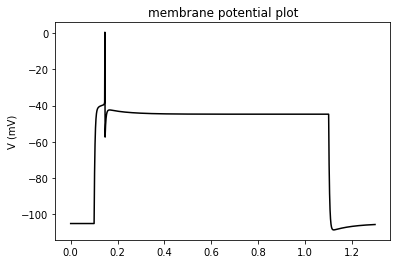
\includegraphics[scale=0.7]{figures/backend_check_files/backend_check_12_10}
\caption[Brian2 simulation of the AdEx model]{Simulated membrane potential trace from the AdEx model at rheobase using the Brian2 simulator.  The action potential waveform itself has been interpolated at the temporal location at which the simulator reported a spike.}
\label{fig:AdEx-Brian2-sim}
\end{center}
\end{figure}

\begin{figure}
\begin{center}
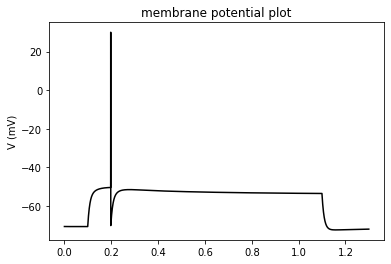
\includegraphics[scale=0.7]{figures/backend_check_files/backend_check_4_2}
\caption[JIT simulation of the AdEx model]{Simulated membrane potential trace from the AdEx model at rheobase using my JIT implementation. In contrast to Fig. \ref{fig:AdEx-Brian2-sim}, the dynamics of the action potential itself arise naturally from the integrated equations, and do not require interpolation.}
\label{fig:AdEx-JIT-sim}
\end{center}
\end{figure}


\subsubsection{Comparison of speed and accuracy vs NEURON}
I also compared the performance of my implementation of the Izhikevich model to the one generated by NEURON from the OpenSourceBrain Izhikevich model NeuroML2 files.
This NEURON implementation has several drawbacks, including: 1) It depends on an external file which must be recompiled each time this project is recreated; 2) The build environment of NEURON is non-trivial; 3) The model implementation code is less generalizable than than the published Izhikevich model itself.
For example, the standard NEURON-NeuroML2 code only covers the Regular-Spiking flavors of this model, and does not support the full range of model parameterizations; 4) Name space conflicts between built-in NEURON parameters and Izhikevich model parameters.  

%\begin{center}
 %   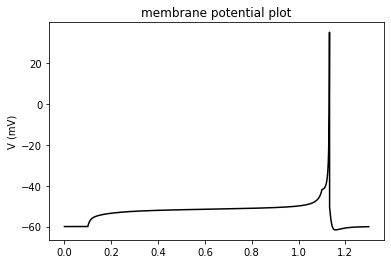
\includegraphics[width=0.7\textwidth,]{chapters/figures/backend_check_files/backend_check_14_2.png}
%    \caption{where is picture}
%\end{center}


%\begin{figure}
%    \centering
%    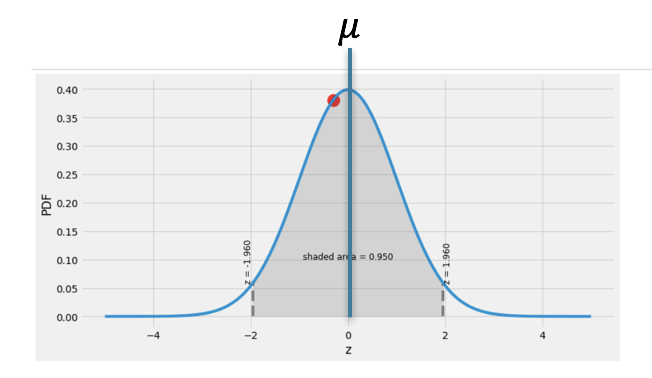
\includegraphics{chapters/normal_distribution}
%    \caption{This is your image%}
%    \label{fig:my_label}
%\end{figure}
%A tool numba JIT

% https://www.overleaf.com/learn/how-to/Images_not_showing_up 
        
The NEURON implementation of the Izhikevich model took $78$ seconds to identify the rheobase current.
In contrast, my implementation identified the rheobase in only $\tilde 0.5 s$.
This represents a very dramatic speed up, and can largely be attributed to overhead associated with initializing successive simulations
Furthermore, my implementation generalizes to all possible parameter values for the Izhikevich model parameters, thus allowing for all of the many diverse spiking behaviors exhibited in the original publication by \cite{izhikevich2003simple}.

%\begin{verbatim}
%  time taken on
%  block 0.6859951019287109 \textbackslash{}n3.3 ms +- 9.79 %$\mu$s per loop (mean +- std. dev. of 2
%  runs, 100 loops each)\textbackslash{}n3.32 ms +- 30.9 us per loop (mean +- std. dev. of 2 runs,
%  100 loops each)\textbackslash{}n3.19 ms +- 10.9 us per loop (mean +- std. dev. of 2 runs, 100
%\end{verbatim}
        
%\subsubsection{Comparison of speed and accuracy vs NEURON for %conductance-based models}
%Could the relatively poor performance of existing implementations 5above be due the use of reduced models?
%I ran similar profiling exercises for a single-compartment %conductance-based model (implementing the Hodgkin-Huxley equations %\cite{rall1962electrophysiology}) to see whether the disparities %above persisted.
%I compared an existing Python implementation for simulation of %this model against the NEURON implementation.
%Conductance-based models took approximately the same amount of
%time ($12.6 s$ XXXX put in exact numbers) to determine the %rheobase as the existing Python
%implementation, suggesting that . XXXX What is this comparison?  %Conductance-based vs Python?

%\begin{center}
%\includegraphics{figures/backend_check_files/backen%d_check_22_2}
%\end{center}

%$ 1.40762329 * pA $
%XXXX Redundant? Hodgkin Huxley Conductance based channels models %took approximately the same amount of time to evaluate the %Rheobase search algorithm as the python implementation.

%The NEURON implementation was slightly faster, and the default parameterization of the model lacked `ringing'', or below threshold oscillations that the Python ODE version had under default conditions.

%This problem in the default parameterization of the python model was later located in the scale or units of capacitance, if default capacitance parameterization is multiplied by 100.0 the problem goes away.

%    \begin{verbatim}
%time taken on block 8.573923826217651
%    \end{verbatim}

\subsubsection{The GLIF Model: a Limited Model}
Although GLIF models are intentionally limited in behavior to below threshold firing dynamics, these models are still relevant to the neuronal modelling community.
I developed a Generalized Leaky Integrate-and-Fire (GLIF) model by manipulating some pre-existing code until it was inter-operable with the NeuronUnit framework. Because GLIF models (the AdEx implementations discussed earlier) do not include spike waveforms imputing spike waveforms is required for broad neuronunit testing. GLIF models were not particularly fast, however GLIF models are very good at predicting the spike timing \cite{teeter2018generalized} (although we did not test this). Including GLIF models was also strategic, these models enjoy usage in the Allen Brain V1 model and we needed to broaden the our perspective of model performance on data driven tests.

%. In practice this class of reduced models is difficult configure without expert knowledge, since it contain more parameters than its competitors, and many of these parameters are vector- rather than scalar-valued.
%Nonetheless, GLIF models were problematic moderately fast with $dt$ set to $5e-3 seconds $ which is 1000 times the recommended 5e-6 seconds, which is offensively slow, and I used these successfully to optimize models against data provided by the Allen Institute (see XXXX section in Results).
%$ Rheobase = 112.5pA $
